
\subsection{Available strategies}

Four classes of observing strategies have been studied in detail:
\begin{itemize}

\item the {\tt OpSim}-based cadences released along with the white
  paper call (11 cadences released in June 2018 plus 4 additional
  simulations released in August), 
  
\item the {\tt OpSim}- and {\tt Feature}-based strategies that were
  available before the white paper call,

\item simulations based on the \altschedsched scheduler proposed by
  Stubbs and Rothchild.  This includes one rolling and another
  non-rolling cadence, plus a non-rolling simulation conducted on a
  larger footprint,

\item finally, we have tested a series of experimental observing
  strategies, based on the new feature-based scheduler (a.k.a.  SLAIR,
  Yoachim et al). These variations were produced by P. Yoachim, the
  main author of SLAIR, based on discussions we had at the summer 2018
  DESC week (CMU) and the 2018 LSST community workshop (Tucson).
\end{itemize}

In table \ref{tab:global_cadence_stats} we report, for each cadence
the total number of exposures per filter. This gives a general idea of
the total open shutter time, and the global filter allocation.  In
table \ref{tab:sn_specific_cadence_stats}, we show SN-specific key
statistics, in particular, the median number of visits in each filter,
for a given location of the sky (e.g. a healpixel), the median cadence
delivered by the observing strategy, the median season duration and
the total footprint of the survey.

The DDF  observations involve a  small number of fields  and $O(10^4)$
SNe. The list of simulated DDF is given in table
\ref{tab:ddf_list} and on figure \ref{fig:ddf_map}. The location of four DDF (referred to as reference fields in the following: \cosmos, \xmmlss, \cdfs~and \elais) has already been chosen by the project. The number of considered DDF ranges from 4 to 9.


\begin{table*}[!htbp]
  \caption{List and location of Deep Drilling Fields observed. "All" stands for all simulations but the ones performed with \altschedsched.}\label{tab:ddf_list}
  \begin{center}
  \begin{tabular}{lcccc}
    \hline
    \hline
    Field name & \opsim~ID & Ra (deg) & Dec(deg) & Observing strategy\\
    \hline
    \hline
    \cosmos & 2786 & 150.36 & 2.84 &All \\
    \xmmlss & 2412 & 34.39 & -5.09 & All \\
    \cdfs & 1427 & 53.00 & -27.44 & All \\
    \elais & 744 & 0.  & -45.52 & All \\
    \spt & 290 & 349.39 & -63.32 & All except feature*\\
    \ddfa & 820 & 119.55 & -43.37 & kraken\_2035\\
    \ddfb & 858 & 187.62 & -42.49 & kraken\_2035\\
    \ddfc & 1200 & 176.63 & -33.15 & kraken\_2035\\
    \ddfd & 2689 & 201.85 & 0.93 & kraken\_2035\\
    \hline
  \end{tabular}
 
  \end{center}
\end{table*}


\begin{figure}[htbp]
\begin{center}
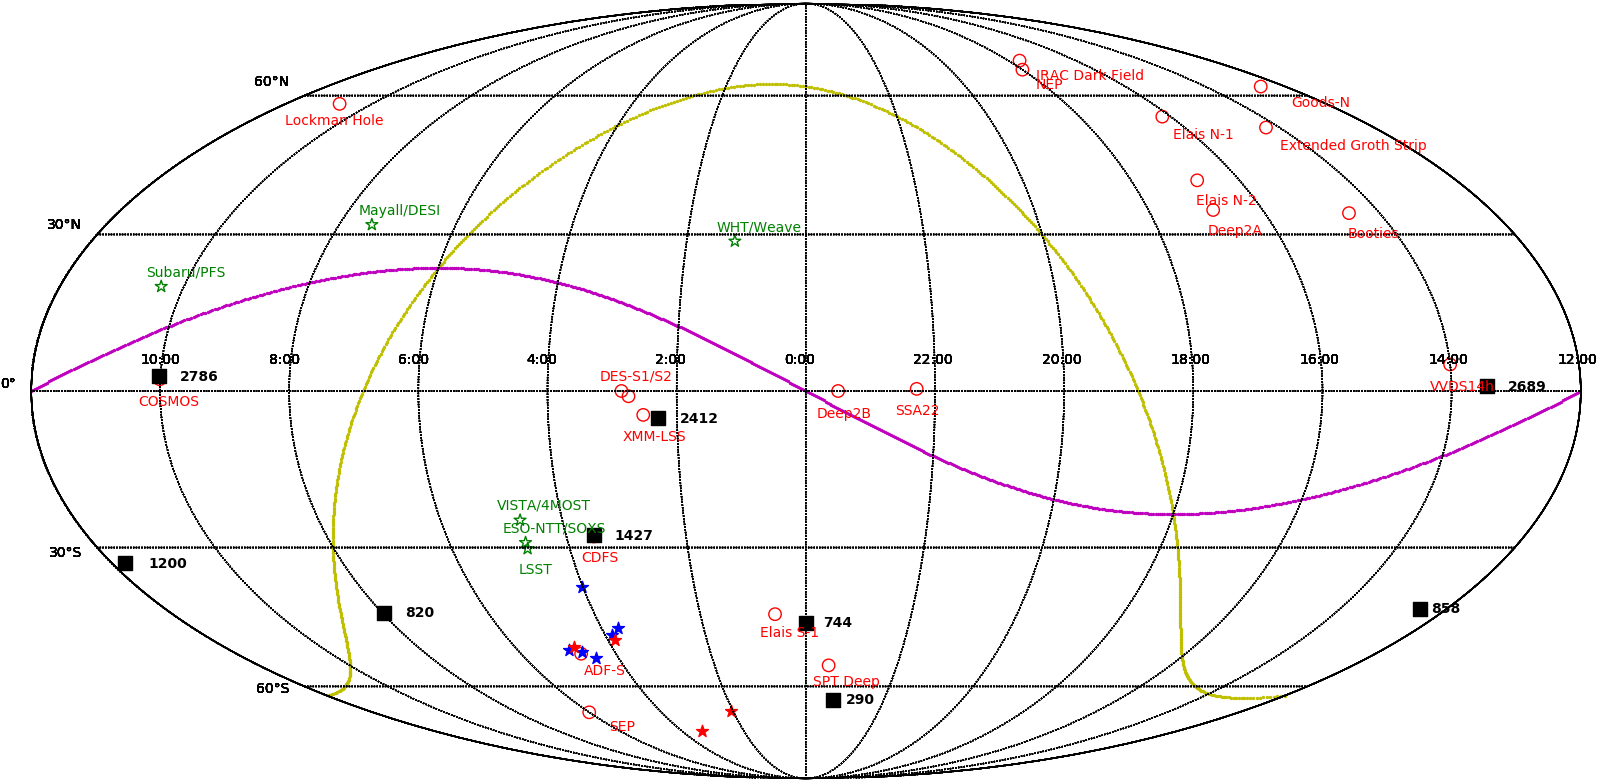
\includegraphics[width=14cm,height=10cm]{overview_strategy/All.png}
\caption{Location of the Deep Drilling fields observed (black squares). Deep fields observed by previous surveys (red circles) and potential candidates for spectroscopic follow-up (green stars) are also mentioned. Yellow and magenta lines represent the Galactic and Ecliptic planes, respectively. Blue and red stars indicate potential deep field locations for EUCLID and WFIRST, respecivelly.}\label{fig:ddf_map}
\end{center}
\end{figure}

DDF observations are composed of sequences of 96 visits\footnote{u band visits are also available but were not considered in the following}  (in a row) in r,g,i,z,y bands (namely 20, 10, 20, 26, 20 visits). This corresponds to a total observing time of about one hour and few minutes if filter changes, slew times and telescope overheads are taken into account.

\subsection{Key properties}

\subsubsection {WFD}
\label{sec:wfd_cadence_key_properties}

\paragraph{Effective SN cadence} What ultimately determines the quality of the SN light curves
and distances is the {\em effective} cadence delivered by the survey,
i.e.  the cadence evaluated after having stacked all the same-band
revisit pairs (or sometimes triplets) performed during one single night. The cadence may be estimated, on each
healpixel, by computing the mean time interval between visits -- after
having excluded the long duration gaps when the healpixel is not
observable.

The effective cadence varies considerably from one observing strategy
to another.  As an illustration, we present on figures
\ref{fig:pontus_2502_effective_cadences},
\ref{fig:altsched_effective_cadences} and
\ref{fig:altsched_rolling_effective_cadences}, we present effective
cadence maps for {\tt Pontus\_2502}, \altsched and \altsched
rolling strategies.  On figure \ref{fig:effective_cadence}, we
report the median cadence in $r$ (computed from similar maps).  The
best effective cadences are delivered by the \altsched like
strategies. We note that there is about a factor 7 between the best
and worst effective cadences.

\begin{figure}
  \begin{center}
    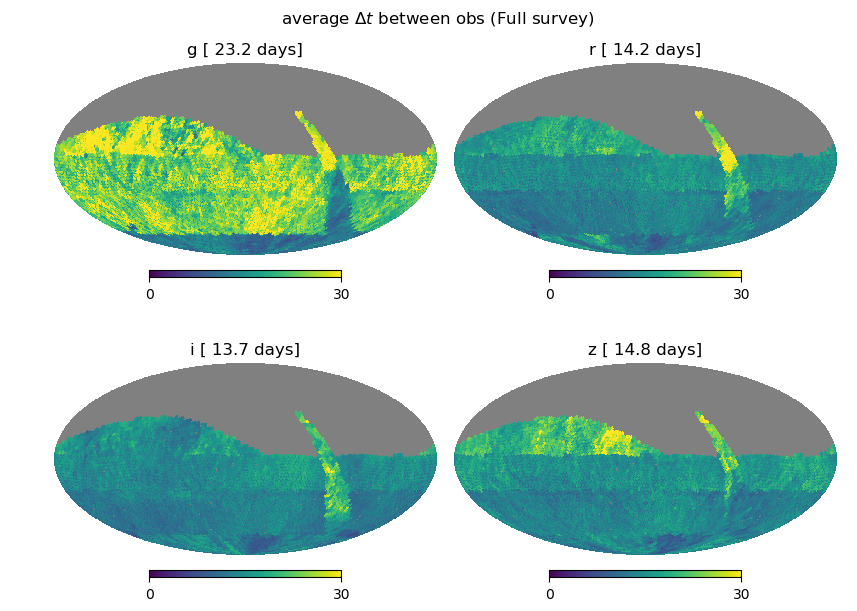
\includegraphics[width=0.8\linewidth]{overview_strategy/pontus_2502_cadence.png}
    \caption{Average $\Delta T$ between observations for {\tt
        Pontus\_2502}, a (slightly rolling) strategy that implements
      same-band visit pairs. }
    \label{fig:pontus_2502_effective_cadences}
  \end{center}
\end{figure}


\begin{figure}
  \begin{center}
    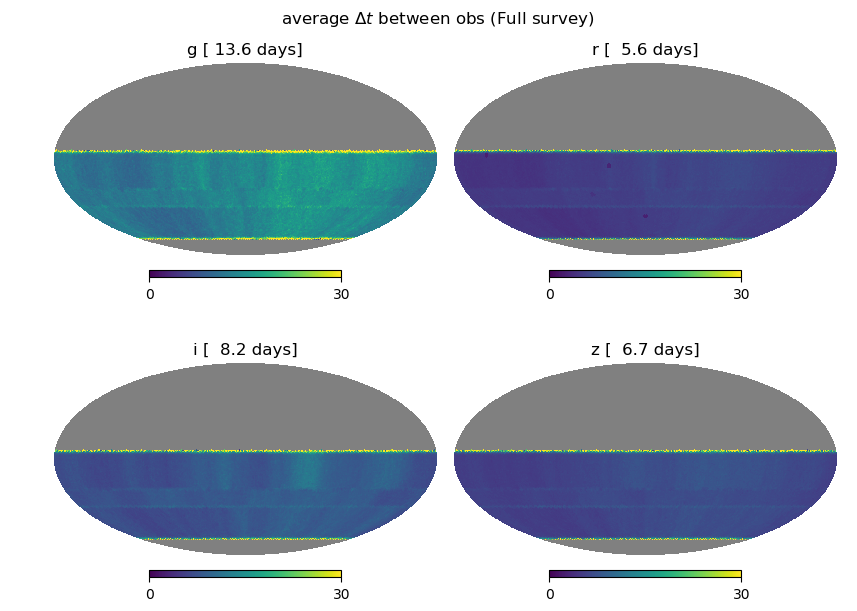
\includegraphics[width=0.8\linewidth]{overview_strategy/altsched_cadence.png}
    \caption{Average $\Delta T$ between observations for \altsched, a strategy that avoid same band visit pairs.}
    \label{fig:altsched_effective_cadences}
  \end{center}
\end{figure}


\begin{figure}
  \begin{center}
    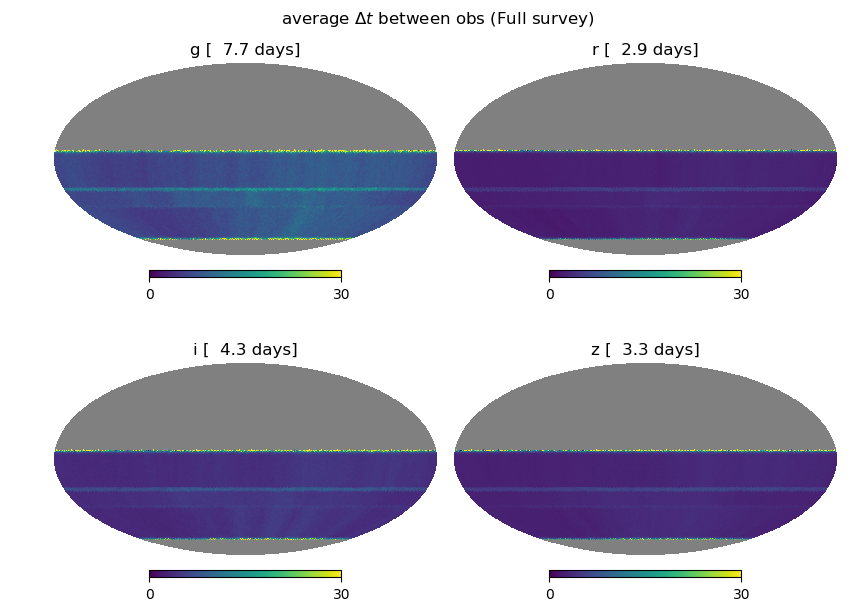
\includegraphics[width=0.8\linewidth]{overview_strategy/altsched_rolling_cadence.png}
    \caption{Average $\Delta T$ between observations for \altsched rolling, a rolling strategy that avoids same band
      visit pairs.}
    \label{fig:altsched_rolling_effective_cadences}
  \end{center}
\end{figure}

\begin{figure}
  \begin{center}
    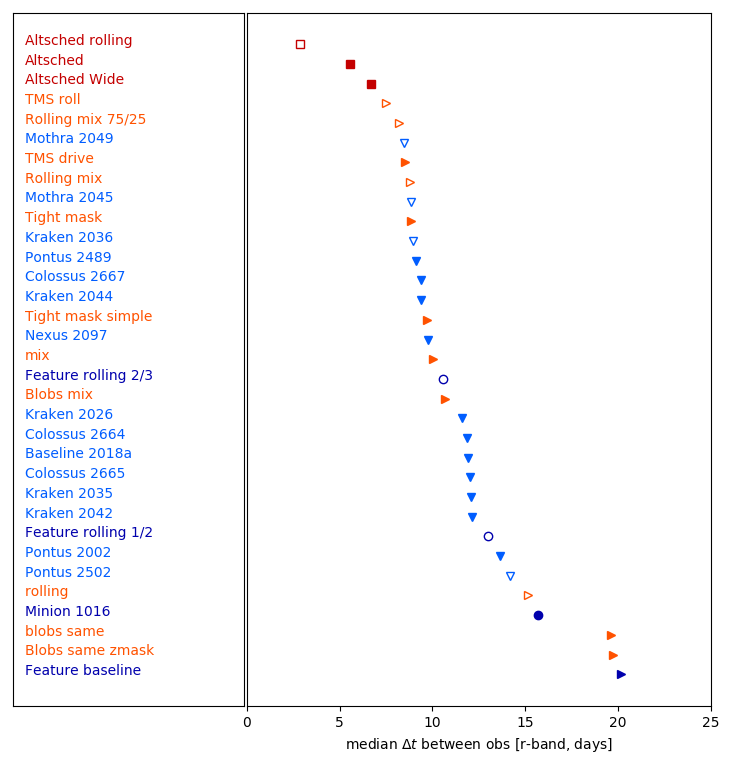
\includegraphics[width=0.8\linewidth]{overview_strategy/cadence.png}
    \caption{Assessment of the effective SN cadence for all
      strategies: median $\Delta T$ between observations (after
      grouping same night observations). \altsched cadences are shown
      in red, \opsim cadences released for the white paper call in
      blue, \slair in orange, and early cadences in deep blue. The
      rolling (resp. non-rolling) cadences are displayed with open
      (resp. solid) markers. }
    \label{fig:effective_cadence}
  \end{center}
\end{figure}

In the remaining of this section, we discuss some of the key design
elements that can explain such large differences.


\paragraph{Global filter allocation} All \opsim and \slair cadences   share the same global filter balance: 
$\sim 7\%, 10\%, 22\%, 22\%, 21\%$ and $18\%$ of the total open shutter time
are allocated to the $u, g, r, i, z$- and $y$ bands respectively.
\altschedsched makes a different choice, based on the fact that the
low-throughput of the LSST camera in $y$, combined with the high sky
brightness in that band limit the impact of $y$-band observations.
About half of the $y$-band observing time is therefore reallocated to
$g$, $r$ and $i$ and $z$ bands, the resulting filter balance is
therefore: 9\%, 11\%, 28\%, 18\% 26\% and 9\% ($ugrizy$ respectively). Of course, having more
observing time in $griz$ can only improve the quality of SN~Ia light curves and distances.


\paragraph{Filter allocation strategy} Another key point, is how the filters are
changed during the night.  In this regard, very different strategies
have been implemented by the various schedulers proposed so far.  This
is illustrated on figure \ref{fig:hourglass_plot_filter_alloc}, which
shows the filter usage for  {\em Pontus 2002} and {\em
  \altsched rolling}.  {\em Pontus 2002} attempts to minimize the
filter changes during a night and in fact keeps observing in the same
filter over several nights.  Conversely, the \altsched family of
cadences attempt to switch for a different filter after each observing
block, so that each revisit of the same field is performed in a
different band.  As we will see below, this has a major impact on the effective cadence
delivered by the survey. As of today, most \opsim cadences released so
far try to minimize the number of filter changes, all \altsched cadences
switch filters after each observing block, and \slair has been
experimenting with both strategies.

\begin{figure}
  \begin{center}
    \subfigure[Pontus 2002]{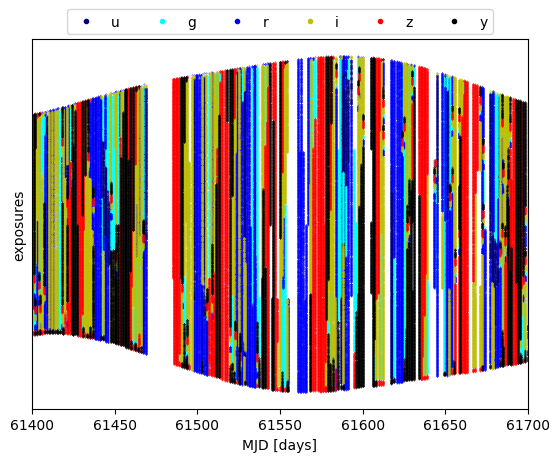
\includegraphics[width=0.48\linewidth]{overview_strategy/pontus_2002_hourglass.png}}
    \subfigure[\altsched rolling]{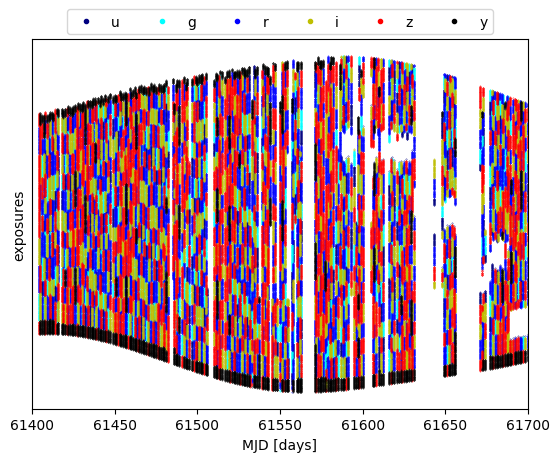
\includegraphics[width=0.48\linewidth]{overview_strategy/alt_sched_rolling_hourglass.png}}
    \caption{Hourglass plots showing the filter usage for two
      different observing strategies. Most \opsim and \slair observing
      strategies released so far tend to minimize the number of filter
      changes. The \altschedsched strategy makes sure that each field is
      observed twice a night in different filter. This results in a
      higher number of filter changes, but is highly beneficial for
      the SN follow-up. }
    \label{fig:hourglass_plot_filter_alloc}
  \end{center}
\end{figure}

\paragraph{The combined effet of visit pairs and filter allocation strategy} In all cadences proposed so far
(except a few simulations, notably {\tt colossus\_2667} and {\tt
  kraken\_2044}) all fields are observed twice a night, 1 to 2 hours
apart, in order to improve the detectability of short term transients
and solar system objects.  Depending on the filter allocation
strategy, this has a strong impact on the sampling quality of the
SN~Ia light curves.  Indeed, SN~Ia luminosities vary significantly
over time scales of 1-2 days.  Same band observations taken during a
given night may therefore be considered as one single visit. When
dealing with a fixed total number of visits per sky direction,
re-observing a field in the same band during a night degrades the SN
light curve sampling by a factor $\sim 2$.

\begin{figure}
  \begin{center}
    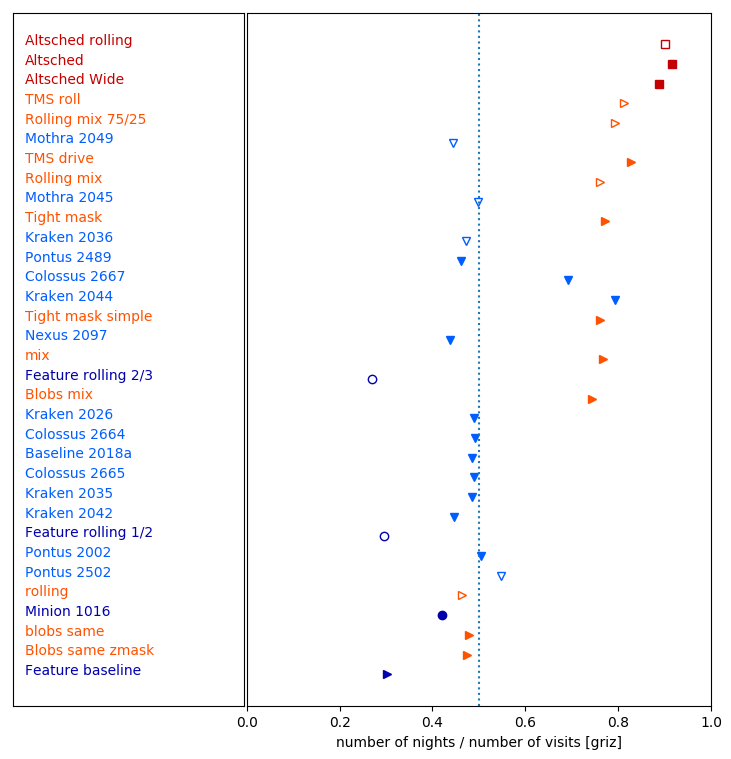
\includegraphics[width=0.8\linewidth]{overview_strategy/night_visit_ratio.png}
    \caption{Number of nights vs. number of visits for the median
      healpixel. We clearly see the effect of the same-band revisit
      strategy.  \altsched cadences are show in red, \opsim WPC in
      blue, \slair in orange, and early cadences in deep blue. The
      rolling (resp. non-rolling) cadences are displayed with open
      (resp. solid) markers. }
    \label{fig:effective_number_of_visits}
  \end{center}
\end{figure}

To estimate that, we compute, for each cadence, the healpix maps
giving the total number of {\em visits} per pixel and the total number
of {\em nights} (several visits per night).  On figure
\ref{fig:effective_number_of_visits}, we show, for each cadence, the
ratio of the median of these maps.  

The survey strategies are sorted according to the effective $r$-band
cadence delivered by the survey (see figure
\ref{fig:effective_cadence}).  We note that most good-cadence
strategies avoid same band revisit pairs. Some strategies however, are
able to compensate.  These are either rolling strategies ({\tt
  Mothra\_2049}, {\tt Mothra\_2045} or {\tt Kraken\_2036}) or by
increasing the total number of visits ({\tt Pontus\_2489}).

All \opsim cadences, except {\tt colossus\_2667} and {\tt
  kraken\_2044} the number of visits is about twice the number of
distinct nights, which is likely to degrade the effective SN cadence
(deeper visits, less often).  All \altsched simulations attempt to
avoid this, as do the recent experiements conducted with \slair.

\paragraph{Season length} This is another feature that may alter the cadence, and the size of the SN sample.
Nearby supernova light curves are less
affected by redshift time dilation, so season duration is not as
crucial as for DDF observations.  However, it is a quantity worth
estimating, in particular to see whether it correlates with the
effective cadence and/or the total size of the SN sample.
Figure \ref{fig:season_length} shows the average season length for
each cadence studied in this work (sorted by $r$-band effective
cadence).  We see considerable differences in season durations (from 130 to 200 days).
Most \opsim and all \altsched strategies manage to observe each field during about
150 consecutive days. The shorter (130 days) and longer (170 days) seasons come mainly from  \slair 
for reasons that have not been elucidated yet. In any case, we do not
note any significant correlation between season duration and cadence.

\begin{figure}
  \begin{center}
    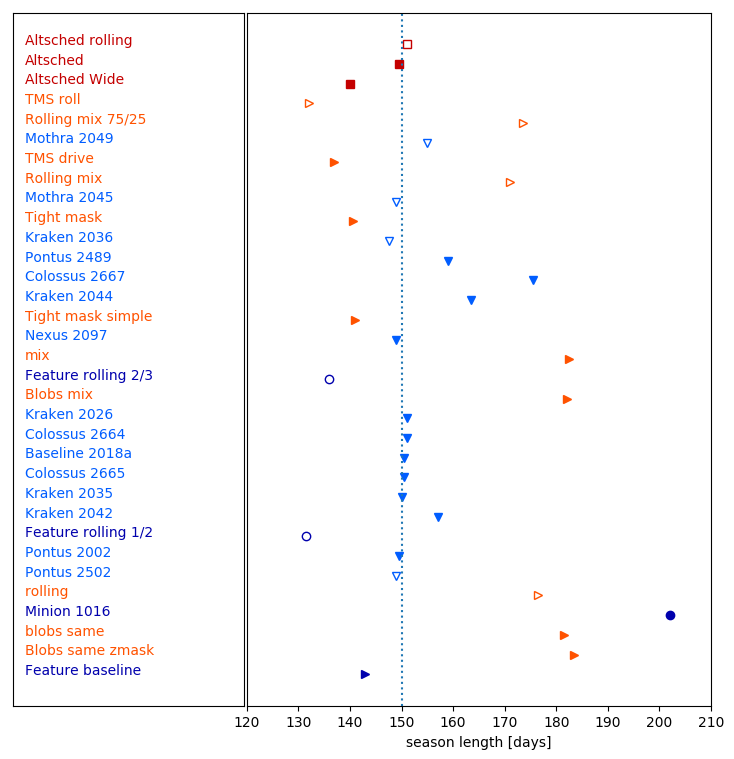
\includegraphics[width=0.8\linewidth]{overview_strategy/season_length.png}
    \caption{Median season duration for each cadence in this
      study. \altsched cadences are show in red, \opsim WPC in blue,
      \slair in orange, and early cadences in deep blue. The rolling
      (resp. non-rolling) cadences are displayed with open
      (resp. solid) markers. }
    \label{fig:season_length}
  \end{center}
\end{figure}

\paragraph{Inter-night gaps}This is another important metric to estimate the ``quality'' of observing strategies. Large gaps between consecutive observations of the same field degrade in a significant way the quality of the supernovae light curves. For each 'healpixel' the fraction of gaps larger than 15 days has been estimated (excluding the very large gaps when the direction is not observable). The conclusion (Figure \ref{fig:large_gaps}) is that \altsched-like cadences tend to have smaller fractions of 15-days gaps (including ''rolling cadences'' which seems quite surprising).

\begin{figure}
  \begin{center}
    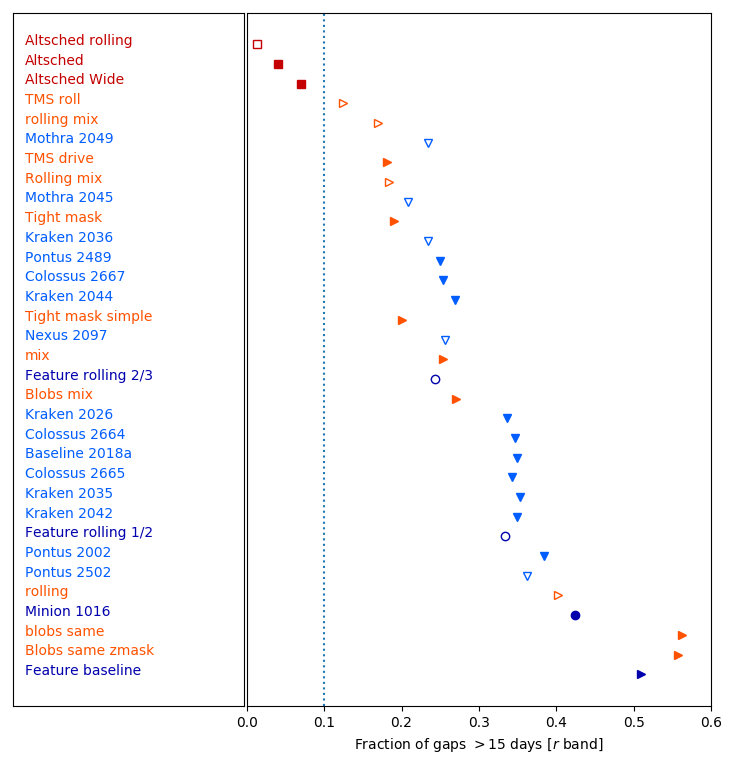
\includegraphics[width=0.8\linewidth]{overview_strategy/cadence_large_gaps.png}
    \caption{Fraction of gaps higher than 15 days (r band).\altsched cadences are show in red, \opsim WPC in blue,
      \slair in orange, and early cadences in deep blue. The rolling
      (resp. non-rolling) cadences are displayed with open
      (resp. solid) markers. }
    \label{fig:large_gaps}
  \end{center}
\end{figure}



\paragraph{} To conclude: we note a very large gap (about a factor 7) between
the best and the worst cadences delivered by the various strategies
released so far.  We will see in the next section, that effective
cadence is the key to maximize the size and depth of the SN sample.
We have discussed a few design elements that help improving the effective
cadence: (1) implementing a rolling strategy (2) change filters often
during the night (3) avoid same band visit pairs.

However, each of these elements taken alone is not
sufficient. Combining all of them has been tried, for example in the
\slair cadences {\tt tms\ roll} and {\tt rolling mix*} and has brought
tremendous improvements with respect to the previous experiments
conducted with this scheduler.  However, the best \slair simulations
are still behind \altschedsched regarding cadence.  On top of the elements
discussed above, it seems that the core of the \altschedsched observing strategy ensures
an extreme regularity of the cadence. This may be explained by the method used by \atlsched~ to observe the sky (see Appendix \ref{sec:opsim_altsched} for more details about differences between \opsim~and \altsched).

\begin{comment}
nrl, 2018-09-27: we still need to estimate (1) the same-filter
 1-day gaps (2) the cadence rms. I think that would help
understanding the difference between the best SLAIR cadences and
Altsched.
\end{comment}



\subsubsection{DDF}


All proposed observing strategies but altsched-like have included DDF.
Plots illustrating some of the key points mentioned above are given on Figures \ref{fig:cosmoscad}-\ref{fig:spt deep_m5} for baseline18a, feature\_baseline\_10yrs, kralen\_2026 and kraken\_2035 observing strategies and for the five to nine above-mentioned DDF. Among these cadences feature\_baseline\_10yrs displays interesting features with respect to supernovae observations for the reference DDF:

\paragraph{Cadence} a median cadence of three days is observed whereas other observing strategies present cadences that may reach up to 14 days. Inter-night gaps are also smaller for \cosmos~and \xmmlss: 10 to 15 days and 5 to 7 days for the first and second maxima respectively whereas  for baseline18a, kralen\_2026 and kraken\_2035 the first (second) maximum is at the level of 18 to 40 (13 to 20) days.  

\paragraph{Season length} feature\_baseline\_10yrs shows the highest season lengths with values around 150 days for \cosmos~and \xmmlss, and 180 days for \cdfs~and \elais~whereas other strategies lead to values of about 130, 140, 120, and 150 days for \cosmos, \xmmlss, \cdfs, and \elais, respectively.

\paragraph{Depth} while median m5-values are compatible among the strategies (the decrease during season 2 for the four fields in  feature\_baseline\_10yrs is due to a known bug in the weather simulations) the coadded m5 depth per season shows clearly that feature\_baseline\_10yrs is a 0.7 (\cosmos), 0.4 (\xmmlss, \cdfs, \elais) magnitude deeper (r-band) survey compared to the others. This results is to be explained by better cadences and longer seasons.
 
Key properties of \spt, \ddfa, \ddfb, \ddfc~and \ddfb~fields are given on Figures \ref{fig:spt deep_cad} to \ref{fig:kraken_m5}.
